\section*{\nr.3 \titthree (10 Punkte)}
\begin{enumerate}[(a)]
\item Eine Skizze der Magnetfeldlinien der Rohre ist durch \vref{fig:rohre} gegeben.
\begin{figure}[htbp]
\centering
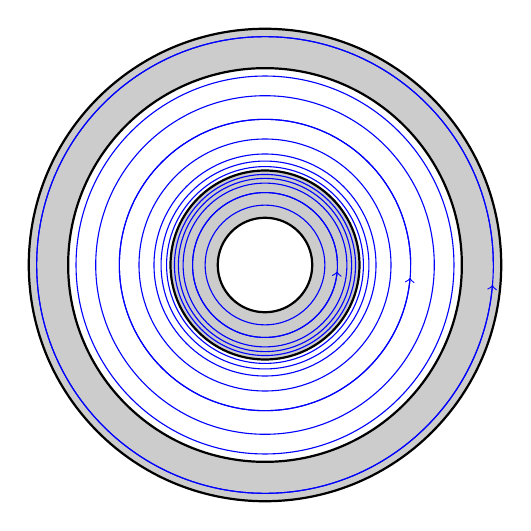
\begin{tikzpicture}

%Rohre
\filldraw[draw=black,thick,fill=gray!40] (0,0) circle[radius=3cm];
\filldraw[draw=black,thick,fill=white] (0,0) circle[radius=2.5cm];
\filldraw[draw=black,thick,fill=gray!40] (0,0) circle[radius=1.2cm];
\filldraw[draw=black,thick,fill=white] (0,0) circle[radius=0.6cm];

%Feldlinien r1-r2

\draw[blue,->] (0.92cm,0) arc[radius=0.92cm,start angle=0, end angle=355];
\draw[blue] (0,0) circle[radius=0.76cm];
\draw[blue] (0,0) circle[radius=0.92cm];
\draw[blue] (0,0) circle[radius=1.04cm];
\draw[blue] (0,0) circle[radius=1.1cm];
\draw[blue] (0,0) circle[radius=1.15cm];

%Feldlinien r2-r3
\draw[blue,->] (1.85cm,0) arc[radius=1.85cm,start angle=0, end angle=355];
\draw[blue] (0,0) circle[radius=1.25cm];
\draw[blue] (0,0) circle[radius=1.32cm];
\draw[blue] (0,0) circle[radius=1.41cm];
\draw[blue] (0,0) circle[radius=1.6cm];
\draw[blue] (0,0) circle[radius=1.85cm];
\draw[blue] (0,0) circle[radius=2.15cm];
\draw[blue] (0,0) circle[radius=2.4cm];

%Feldlinien r3-r4
\draw[blue] (0,0) circle[radius=2.9cm];
\draw[blue,->] (2.9cm,0) arc[radius=2.9cm,start angle=0, end angle=355];

\end{tikzpicture}
\caption{Magnetfeldlinien in stromdurchlossener Anordnung. Sie zeigen gegen den Uhrzeigersinn, wenn der Strom im inneren Rohr aus der Zeichenebene heraus und im äußeren Rohr in die Zeichenebene hineinfließt.}
\label{fig:rohre}
\end{figure}

\item 
Im Folgenden werten wir willkürlich Magnetfelder, die entgegen des Uhrzeigersinns in \vref{fig:rohre} laufen, positiv, andere negativ.

Aus Symmetriegründen gilt für einen Kreisweg $C$ mit Radius $r$ entlang der Feldlinien folgendes Wegintegral:
\begin{equation}
\oint_C {\vec{B}\cdot\mathrm{d}\vec{s}} = \int_C B\mathrm{d}s = \int_0^{2\pi} {Br\mathrm{d}\phi} = 2\pi r B
\label{eq:wegint}
\end{equation}

Für den Bereich $0<r<r_1$ gilt nach dem Ampère'schen Durchflutungssatz
\begin{equation}
\oint_C \vec{B}\cdot\mathrm{d}\vec{s} = 0,
\end{equation} 
da kein Strom durch den Weg eingeschlossen ist. Mit \vref{eq:wegint} folgt $B=0$.

Für den Bereich $r_1 < r < r_2$ nehmen wir an, dass die Stromdichte im Rohr homogen ist. Dann folgt:
\begin{equation}
\oint_C \vec{B}\cdot\mathrm{d}\vec{s} = \mu_0 I_0 \frac{\pi r^2-\pi r_1^2}{r_2^2-r_1^2} = \mu_0 I_0 \frac{r^2-r_1^2}{r_2^2-r_1^2}
\end{equation}
Mit \vref{eq:wegint} folgt $B=\frac{\mu_0 I_0}{2\pi r} \frac{r^2-r_1^2}{r_2^2-r_1^2}$.

Für $r_2 < r < r_3$ gilt:
\begin{equation}
\oint_C \vec{B}\cdot\mathrm{d}\vec{s} = \mu_0 I_0
\end{equation}
Also gilt nach \vref{eq:wegint} $B=\mu_0 I_0/(2\pi r)$. 

Im Bereich $r_3 < r < r_4$ gilt:
\begin{equation}
\oint_C \vec{B}\cdot\mathrm{d}\vec{s} = \mu_0 I_0 - \mu_0 I_0 \frac{\pi r^2-\pi r_3^2}{\pi r_4^2 - \pi r_3^2}= \mu_0 I_0 \frac{r_4^2-r^2}{r_4^2-r_3^2}
\end{equation}
Für $B$ folgt nach \vref{eq:wegint} dann $B=\frac{\mu_0 I_0}{2\pi r} \frac{r_4^2-r^2}{r_4^2-r_3^2}$.

Außerhalb der Rohre, für den Bereich $r>r_4$, gilt:
\begin{equation}
\oint_C \vec{B}\cdot\mathrm{d}\vec{s} = \mu_0 I_0 -\mu_0 /_0 = 0,
\end{equation}
wodurch nach \vref{eq:wegint} schließlich $B=0$ folgt.

\item Der Verlauf von $B(r)$ ist in \vref{fig:magnetfeld} dargestellt.
\begin{figure}[htbp]
\centering
\begin{tikzpicture}
%Koordinatensystem und Beschriftungen
\draw[<->] (0,5)node[left]{$B$} -- (0,0) -- (6.5,0) node[right]{$r$};
\draw (1,-0.2)node[below]{$r_1$} -- (1,0.1);
\draw (2,-0.2)node[below]{$r_2$} -- (2,0.1);
\draw (4,-0.2)node[below]{$r_3$} -- (4,0.1);
\draw (5,-0.2)node[below]{$r_4$} -- (5,0.1);
%Graphen
\begin{scope}[color=orange!70!black, very thick]
\draw (0,0) -- (1,0);
\draw plot[id=r12,samples=100,domain=1:2] function{8.0/3.0*(x*x-1.0)/x};
\draw plot[id=r23,samples=100,domain=2:4] function{8/x};
\draw plot[id=r34,samples=100,domain=4:5] function{8.0/9.0*(25.0-x*x)/x};
\draw (5,0) -- (6,0);
\end{scope}
\end{tikzpicture}
\caption{Betrag der magnetischen Flussdichte $B$ als Funktion des Radius $r$.}
\label{fig:magnetfeld}
\end{figure}

\end{enumerate}